\section{Bosonic cumulants}
\begin{frame}
    \frametitle{Results for 14e19o}
    \begin{figure}
        \centering
        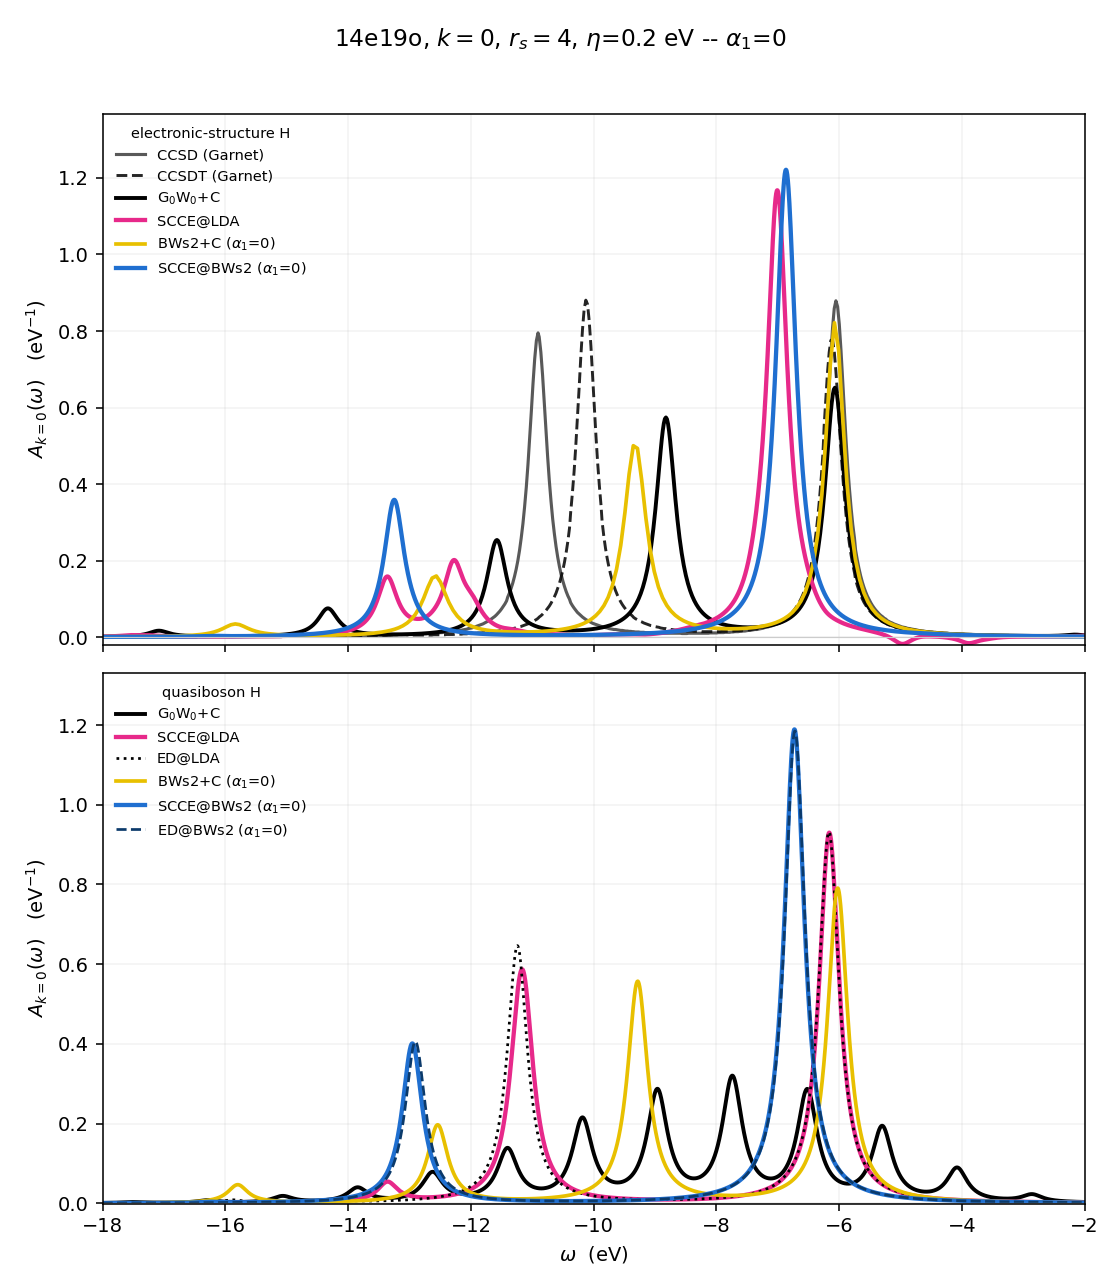
\includegraphics[width=0.6\textwidth]{26/9/9-15/k0_14e19o_alpha0_scce_all.png}
\end{figure}
\end{frame}
\begin{frame}
    \frametitle{Results for 14e19o}
    \begin{figure}
        \centering
        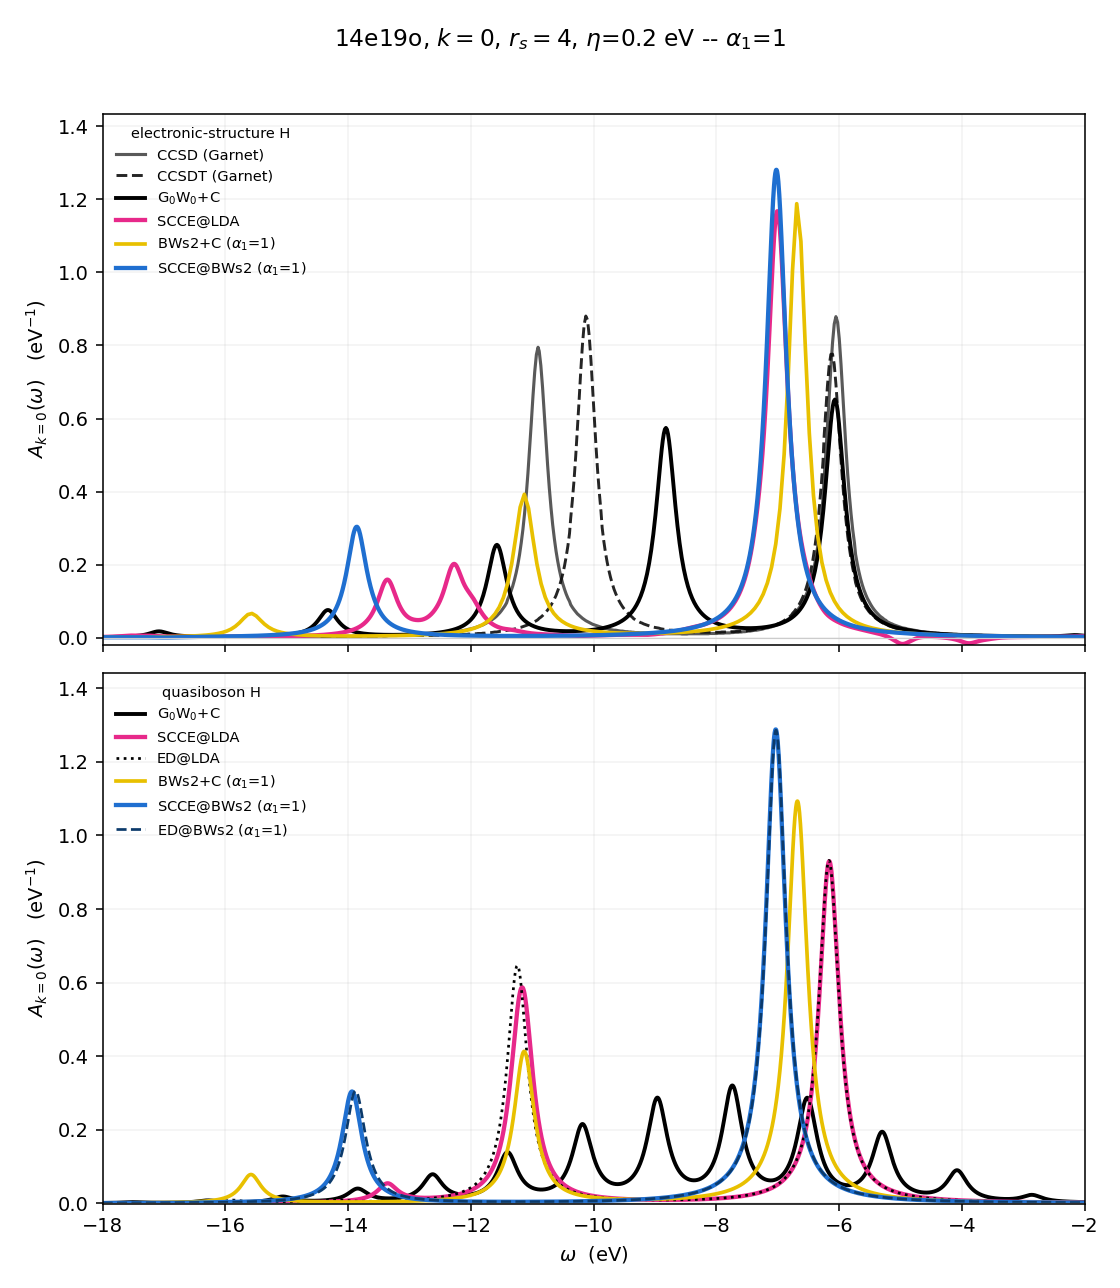
\includegraphics[width=0.6\textwidth]{26/9/9-15/k0_14e19o_alpha1_scce_all.png}
\end{figure}
\end{frame}
\begin{frame}
    \frametitle{Results for 14e19o}
    \begin{figure}
        \centering
        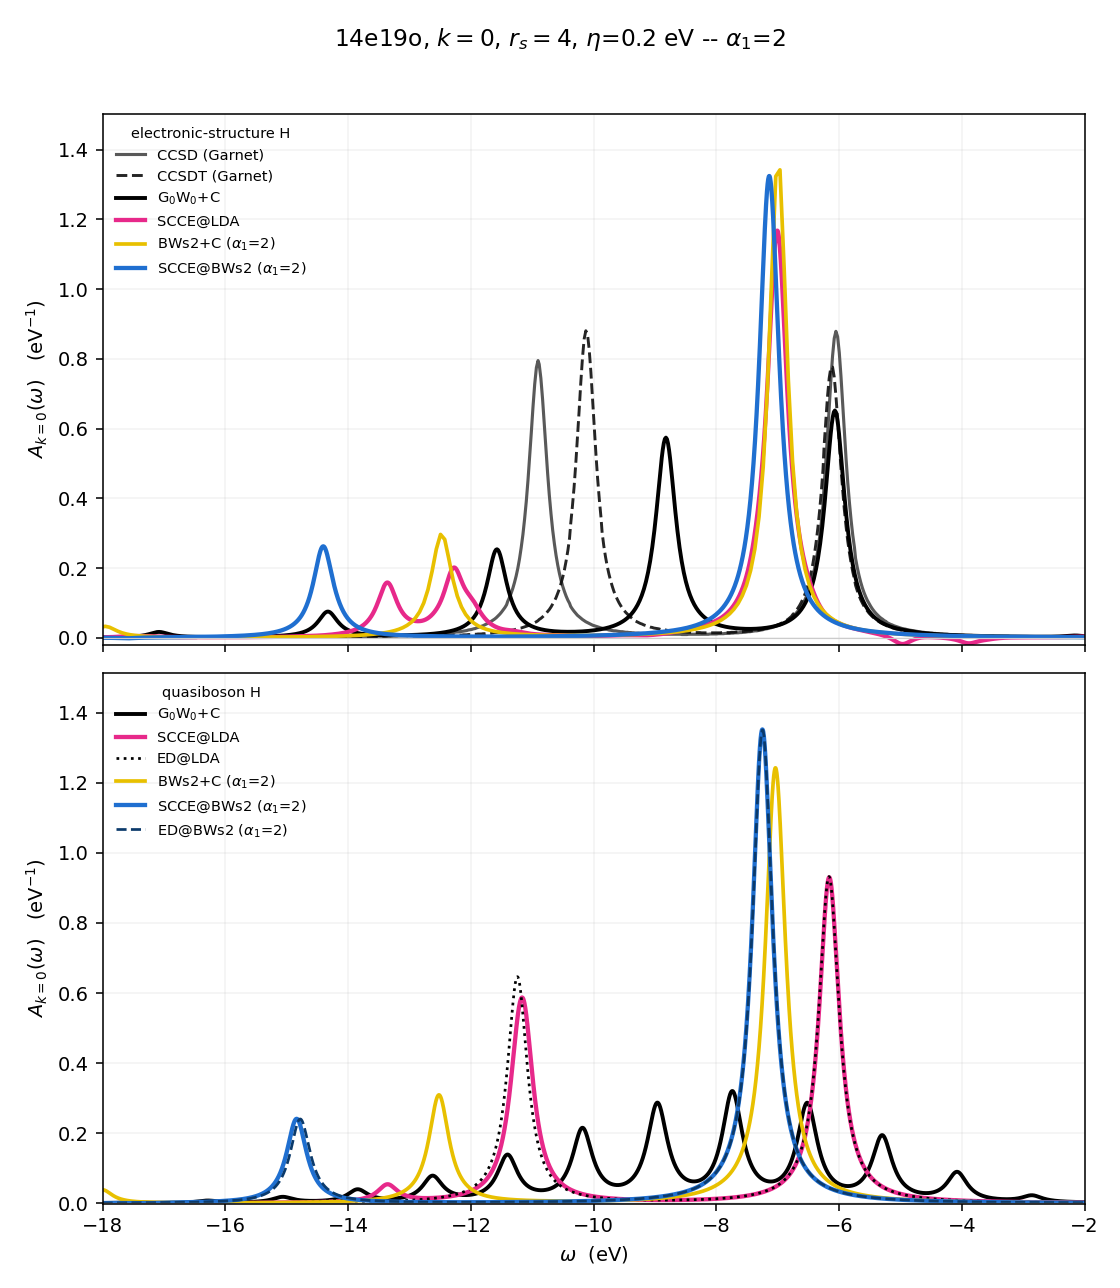
\includegraphics[width=0.6\textwidth]{26/9/9-15/k0_14e19o_alpha2_scce_all.png}
\end{figure}
\end{frame}
\begin{frame}
    \frametitle{Results for 14e19o}
    \begin{figure}
        \centering
        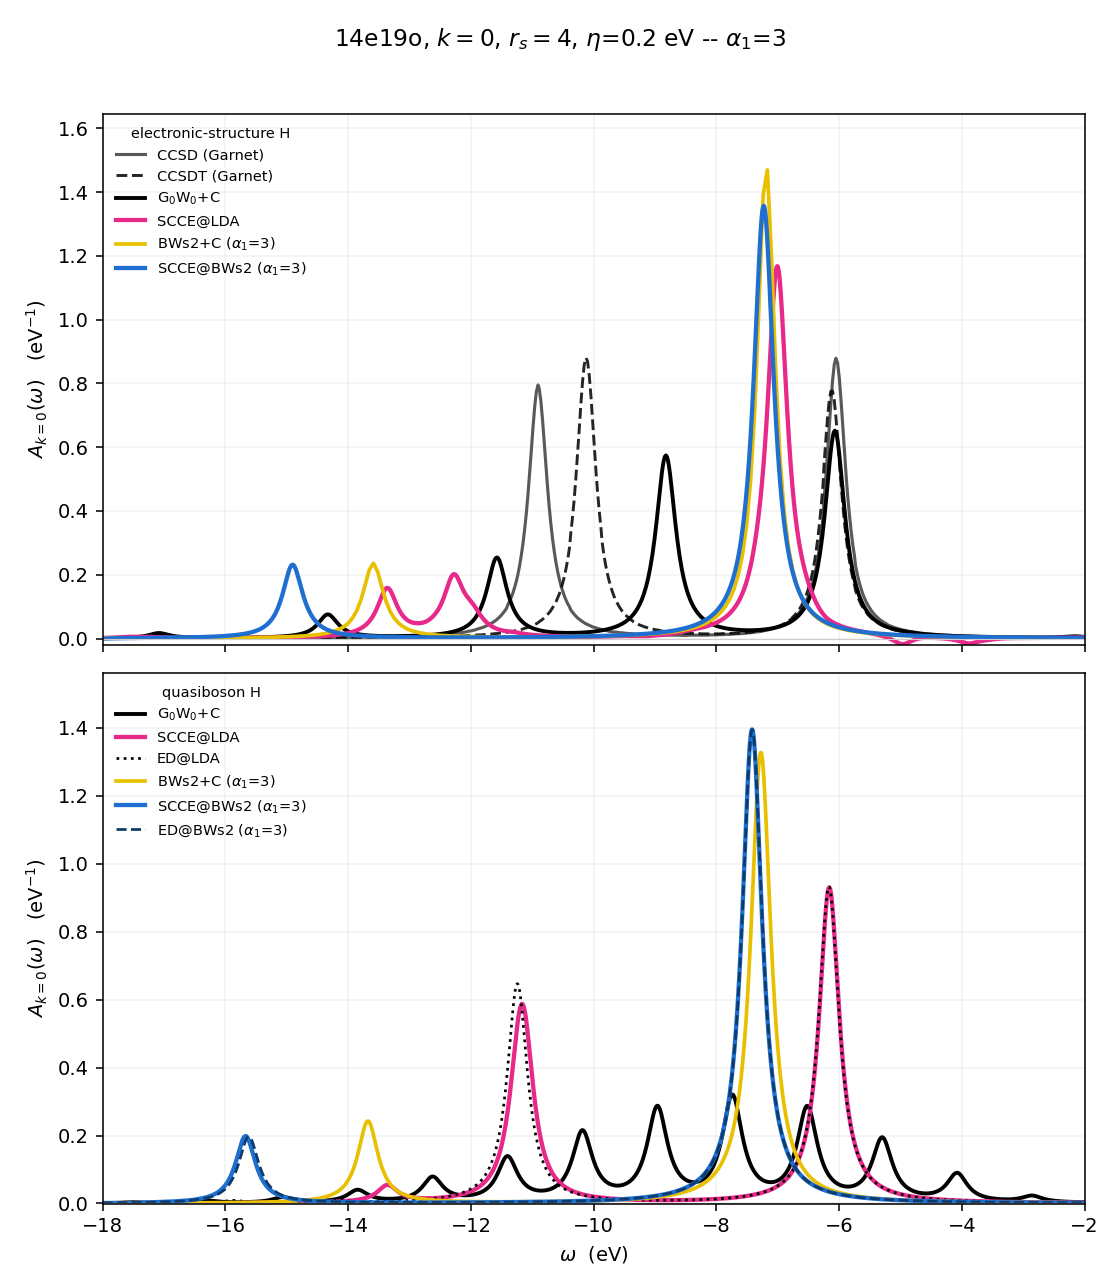
\includegraphics[width=0.6\textwidth]{26/9/9-15/k0_14e19o_alpha3_scce_all.png}
\end{figure}
\end{frame}
\begin{frame}
    \frametitle{Results for 14e19o}
    \begin{figure}
        \centering
        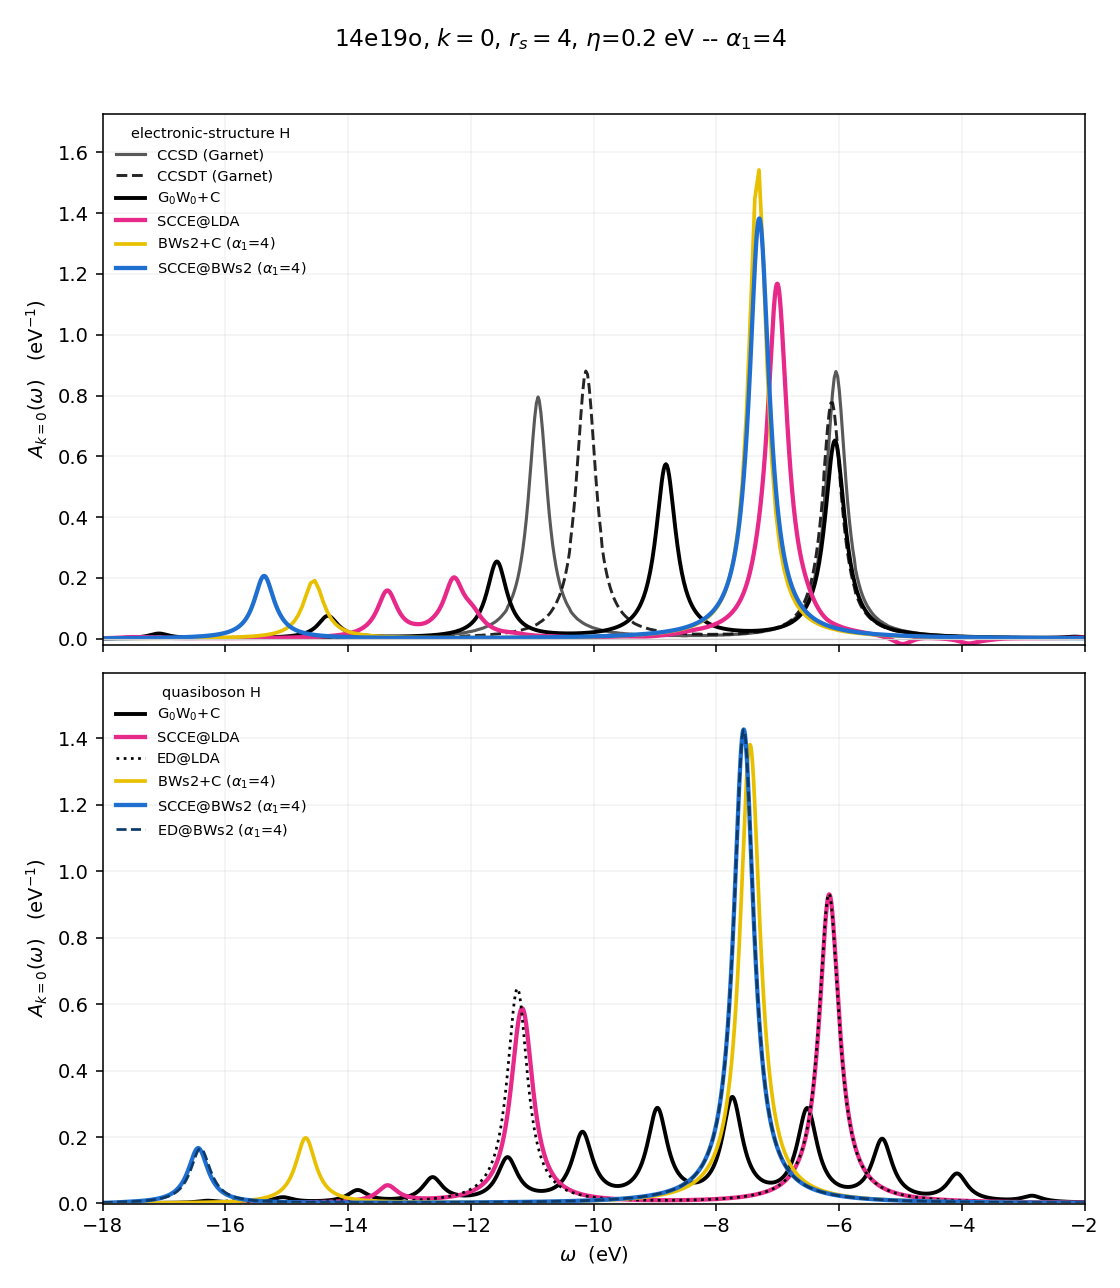
\includegraphics[width=0.6\textwidth]{26/9/9-15/k0_14e19o_alpha4_scce_all.png}
\end{figure}
\end{frame}
\begin{frame}
    \frametitle{Results for 114e485o}
    \begin{figure}
        \centering
        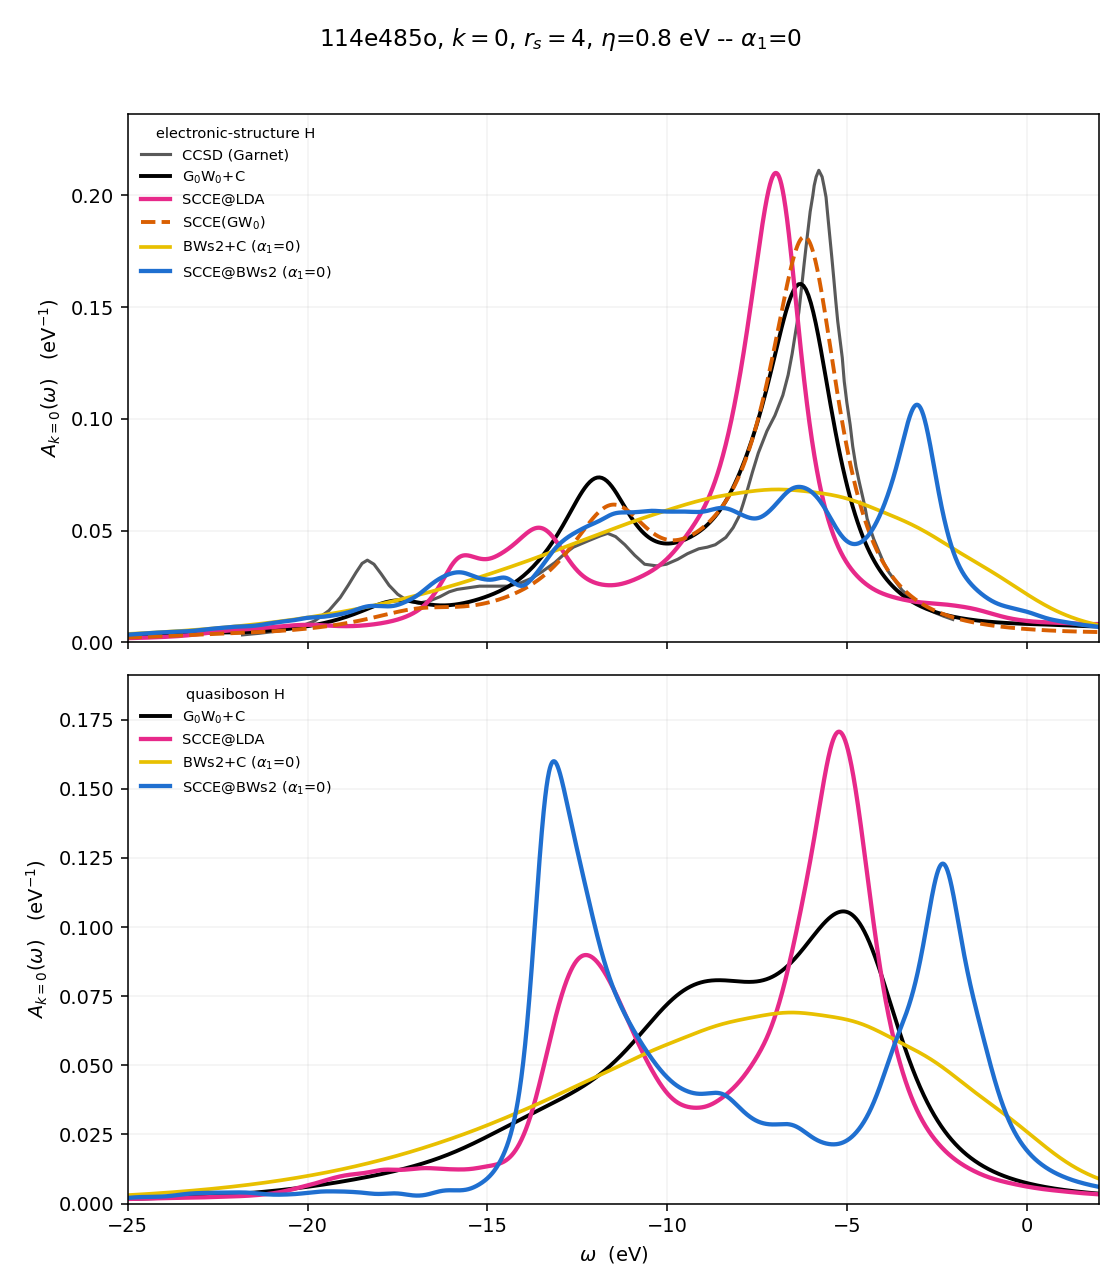
\includegraphics[width=0.6\textwidth]{26/9/9-15/k0_114e485o_alpha0_scce_all.png}
\end{figure}
\end{frame}
\begin{frame}
    \frametitle{Results for 114e485o}
    \begin{figure}
        \centering
        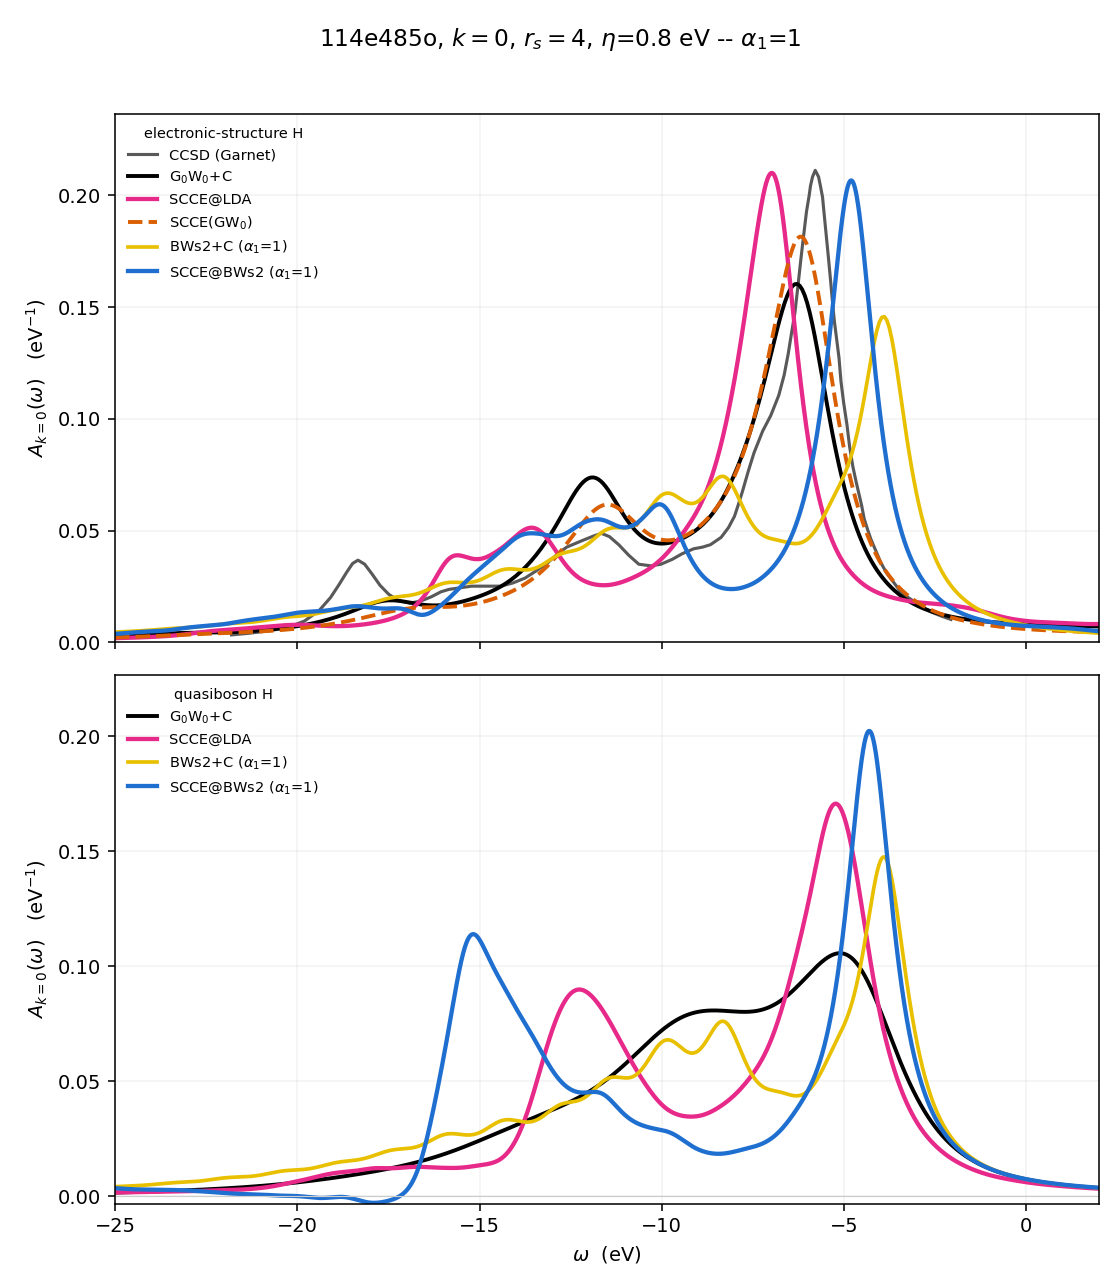
\includegraphics[width=0.6\textwidth]{26/9/9-15/k0_114e485o_alpha1_scce_all.png}
\end{figure}
\end{frame}
\begin{frame}
    \frametitle{Results for 114e485o}
    \begin{figure}
        \centering
        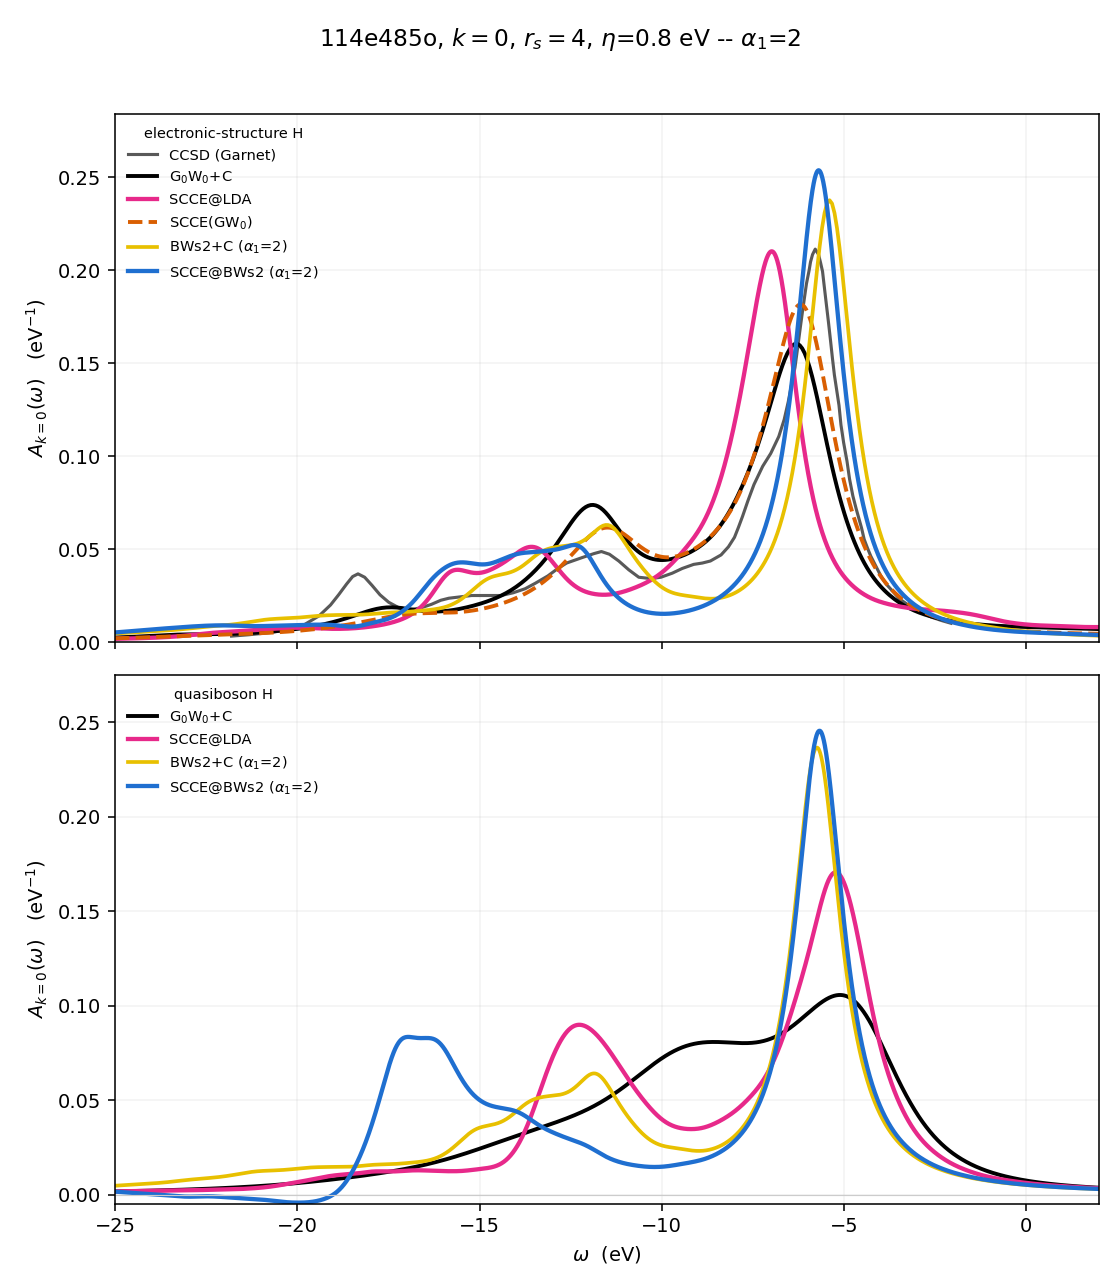
\includegraphics[width=0.6\textwidth]{26/9/9-15/k0_114e485o_alpha2_scce_all.png}
\end{figure}
\end{frame}
\begin{frame}
    \frametitle{Results for 114e485o}
    \begin{figure}
        \centering
        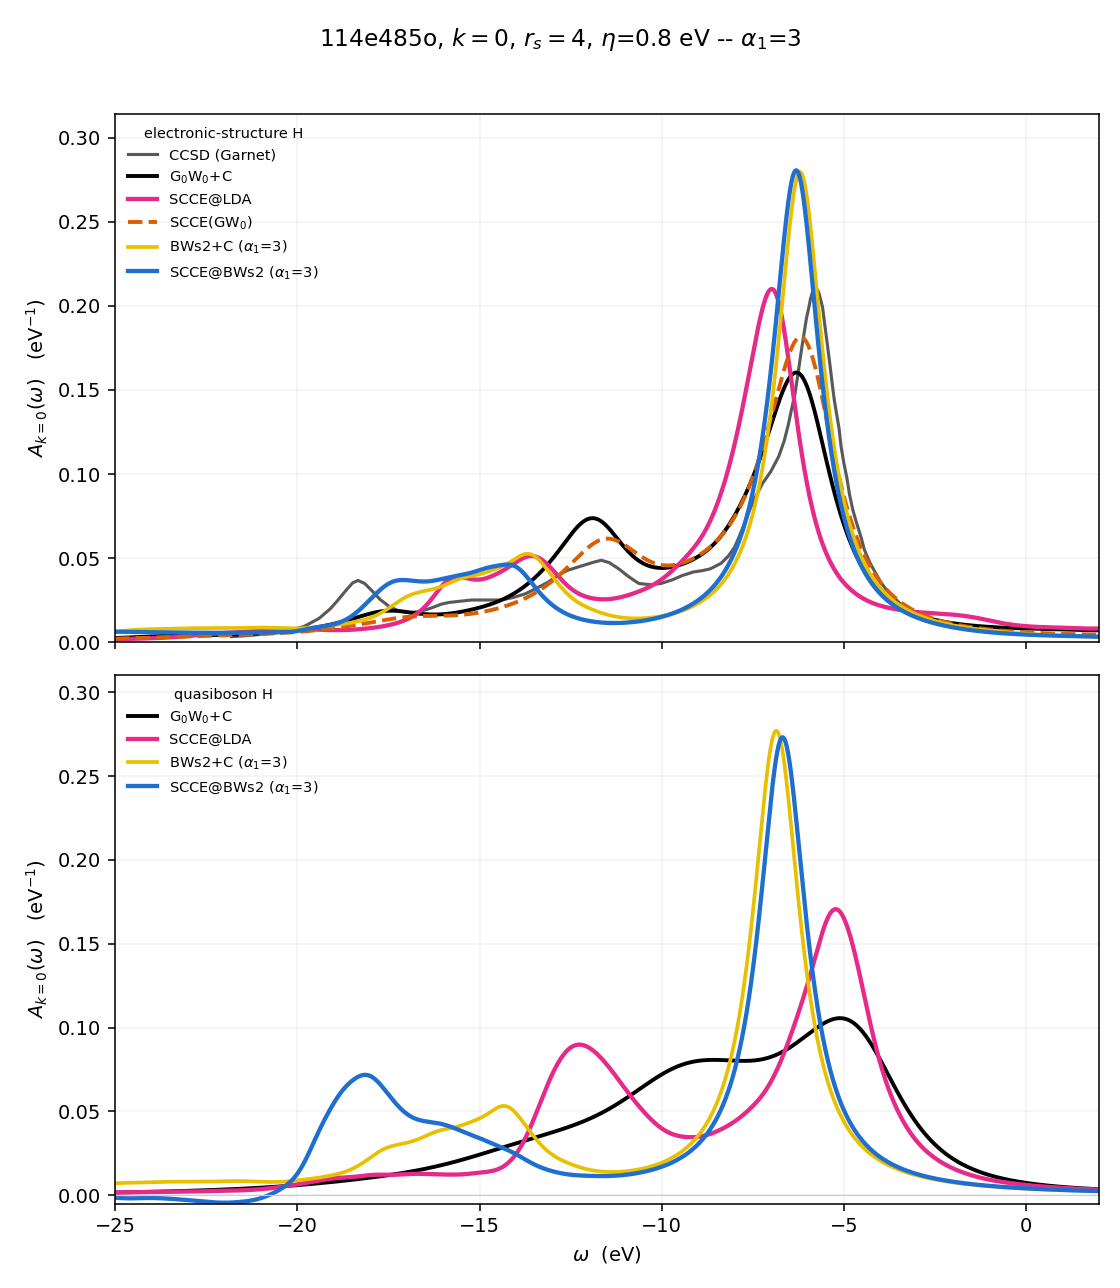
\includegraphics[width=0.6\textwidth]{26/9/9-15/k0_114e485o_alpha3_scce_all.png}
\end{figure}
\end{frame}
\begin{frame}
    \frametitle{Results for 114e485o}
    \begin{figure}
        \centering
        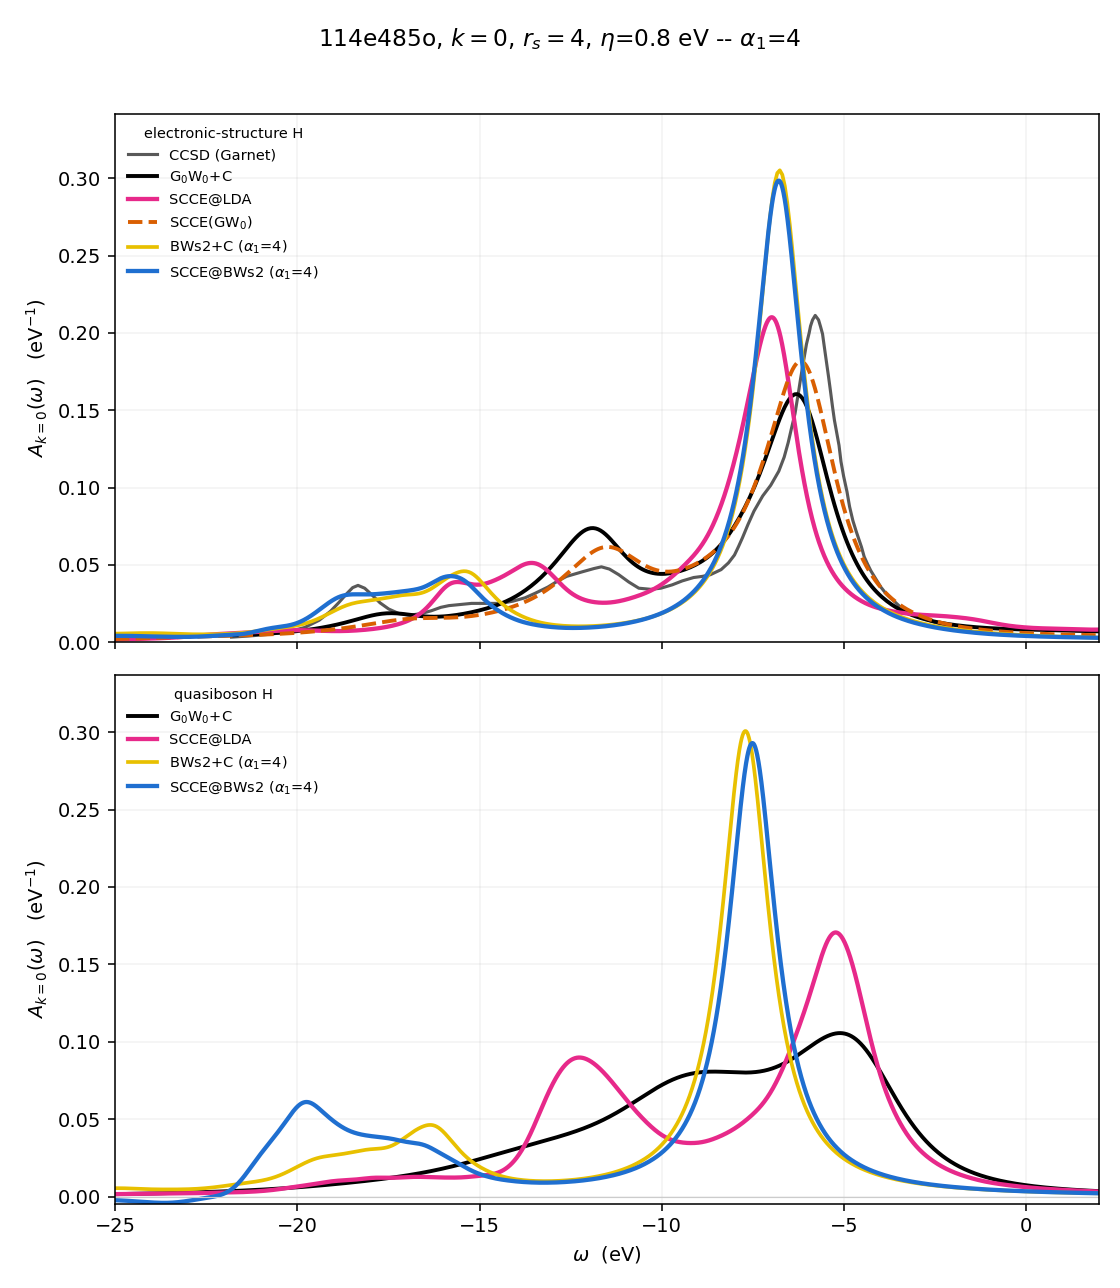
\includegraphics[width=0.6\textwidth]{26/9/9-15/k0_114e485o_alpha4_scce_all.png}
\end{figure}
\end{frame}

\section{Fermionic cumulants}
\begin{frame}
    \frametitle{Theory}
We can solve
\begin{equation}
\frac{d\mathbf{C}(t)}{dt}
=
\mathbf{F}[\mathbf{C}](t)
\end{equation}
with
\begin{equation}
\mathbf{C}(t)
=
\left(
\{C_{\bm{a}}^{+}(t)\}_{\bm{a}\in\mathcal{V}},
\{C_{\bm{i}}^{-}(t)\}_{\bm{i}\in\mathcal{O}}
\right).
\end{equation}
\end{frame}
\begin{frame}
    \frametitle{The coupled VIDEs}
 We determine the Green's functions for particles and holes as $G_{\bm{a}}(t)=-i e^{-i\epsilon_{\bm{a}}^{\rm ref}t+C_{\bm{a}}^{+}(t)-\eta t}$ and $G_{\bm{i}}(t)=-i e^{-i\epsilon_{\bm{i}}^{\rm ref}t+C_{\bm{i}}^{-}(t)-\eta t}$, respectively. \pause
For particles, we have
\begin{align}
\frac{dC_{\bm{a}}^{+}(t)}{dt}
&=
-i\mathcal{C}_{\bm{a}}
-
\sum_{c\nu}
\mathcal{K}_{\bm{a}c\nu}
\int_0^t d\tau\,
e^{i\Delta_{\bm{a}c\nu}^{(+)}(t-\tau)}
e^{\Phi_{\bm{a}c\nu}(t,\tau)}.
\end{align}\pause
For holes, we have
\begin{align}
\frac{dC_{\bm{i}}^{-}(t)}{dt}
&= - i\mathcal{C}_{\bm{i}}
-
\sum_{k\nu}
\mathcal{K}_{\bm{i}k\nu}
\int_0^t d\tau\,
e^{i\Delta_{\bm{i}k\nu}^{(-)}(t-\tau)}
e^{\Psi_{\bm{i}k\nu}(t,\tau)}.
\end{align}
\end{frame}
\begin{frame}
    \frametitle{LDA reference}
Here, $\mathcal{C}_{\bm{p}}=0$ and $\epsilon_{\bm{p}}^{\rm ref}=|\bm{p}|^2/2 + \Sigma_{\bm{p}}^x$. \pause Note that we never explicitly update the exchange self-energy, as in Holm. \pause Also, we have
\begin{align}
\Delta_{\bm{p}k,\nu}^{(-)}
&=
\epsilon_{\bm{p}}^{\rm LDA}
-\epsilon_k^{\rm LDA}
+
\omega_{\nu}^{\rm pl}
, \quad
\Delta_{\bm{p}c,\nu}^{(+)}
=
\epsilon_{\bm{p}}^{\rm LDA}
-\epsilon_c^{\rm LDA}
-
\omega_{\nu}^{\rm pl}
\end{align}\pause
and (where $\bm{q}$ is the momentum imparted by plasmon mode $\nu$)
\begin{align}
\mathcal{K}_{\bm{p}k\nu}
&=
\left|g_\nu^{\rm pl}(\bm{p},\bm{q})\right|^2, \quad \bm{p}-\bm{q}\in\mathcal{O}
,\quad 
\mathcal{K}_{\bm{p}c\nu}
=
\left|g_\nu^{\rm pl}(\bm{p},\bm{q})\right|^2, \quad \bm{p}-\bm{q}\in\mathcal{V}
\end{align} \pause
% \mathcal{L}_{\bm{k}i\nu}
% &=
% \left|g_\nu^{\rm pl}(\bm{k},\bm{q})\right|^2, \quad \bm{k}-\bm{q}\in\mathcal{O}
% ,\\
% \mathcal{L}_{\bm{k}a\nu}
% &=
% \left|g_\nu^{\rm pl}(\bm{k},\bm{q})\right|^2, \quad \bm{k}-\bm{q}\in\mathcal{V}
% \end{align}
We used the LDA single-particle energies $\epsilon_{\bm{k}}^{\rm LDA}$ along with the dRPA@LDA excitation energies $\omega_{\nu}^{\rm pl}$ and transition densities $g_\nu^{\rm pl}(\bm{k},\bm{q})$. \pause
Here we take 
\begin{align}
\Psi_{\bm{p}q\nu}(t,\tau)
&=
% -C_i^{-}(t)
% +C_i^{-}(\tau)
% +C_j^{-}(t)
% -C_j^{-}(\tau)
% \nonumber\\
% &\quad
+C_p^{-}(t)
-C_p^{-}(\tau)
+C_q^{-}(t)
-C_q^{-}(\tau),
\end{align}
given that we freeze the plasmon modes at the dRPA@LDA level. \pause This means that if we choose the dRPA@LDA reference, we are forced to do bosonic cumulants. And so we only have one VIDE to solve, if we want the electron-removal spectral function of the state at the bottom of the band.
\end{frame}
\begin{frame}
    \frametitle{BW reference}
Here, $\tilde{\varepsilon}_{{k}}$ denote the BWs2 single-particle energies. \pause We can try $\nu\equiv jb$ if we want to do fully fermionic cumulants. \pause Then, $\mathcal{C}_{\bm{p}}=-\alpha W_{\bm{p}\bm{p}}$, where $W_{\bm{p}\bm{p}}=\Theta(|\bm{k}_F| - |\bm{p}|)\Sigma^{2p1h}_{\bm{p}\bm{p}}(\tilde{\varepsilon}_{\bm{p}})$\pause and $\epsilon_{\bm{p}}^{\rm ref}=\tilde{\varepsilon}_{\bm{p}}$.\pause Also,
we have
\begin{align}
\Delta_{\bm{p}k\nu}^{(-)}
&=
\tilde{\varepsilon}_{\bm{p}}
-\tilde{\varepsilon}_k
+{\varepsilon_b^{\rm HF}} - \tilde{\varepsilon}_j, \quad \Delta_{\bm{p}c\nu}^{(+)}
=
\tilde{\varepsilon}_{\bm{p}}
-\epsilon_c^{\rm HF}
-{\varepsilon_b^{\rm HF}} + \tilde{\varepsilon}_j
% , \quad
% \Delta_{\bm{k}a,\nu}^{(+)}
% =
% \tilde{\varepsilon}_{\bm{k}}
% -\epsilon_a^{\rm HF}
% -
% \tilde{\Omega}_{\nu}
\end{align} \pause
and second-order Coulomb interaction kernels defined by $\mathcal K_{pqrs}=
(pr|qs)
\left[
2(pr|qs)-(pq|rs)
\right]$.\pause We can take 
\begin{align}
\Psi_{\bm{p}k\nu}(t,\tau)
&=
-C_p^{-}(t)
+C_p^{-}(\tau)
+C_k^{-}(t)
-C_k^{-}(\tau) - C_b^{+}(t) + C_b^{+}(\tau) + C_j^{-}(t) - C_j^{-}(\tau) \\
\Psi_{\bm{p}c\nu}(t,\tau)
&=
-C_p^{+}(t)
+C_p^{+}(\tau)
+C_c^{+}(t)
-C_c^{+}(\tau) + C_b^{+}(t) - C_b^{+}(\tau) - C_j^{-}(t) + C_j^{-}(\tau)
\end{align}
\end{frame}